\documentclass[]{article}

\usepackage{tikz}
\usepackage{amsmath}
\usepackage{amsfonts}
\usepackage{amssymb}
\usepackage{tkz-base}
\usepackage{tkz-euclide}

\usetikzlibrary{svg.path}
\usetikzlibrary{arrows}
\usetikzlibrary{shapes.geometric,calc}

%opening
\title{Jacobians in the Force Domain}
\author{Craig Carignan\\Glen Henshaw}

\begin{document}

\maketitle

\begin{abstract}

\end{abstract}

\section{Intro}
Let's consider moment and force propagation through a link, instead of angular and linear velocity propagation.

In the static case:

\begin{figure}[!h]
\centering
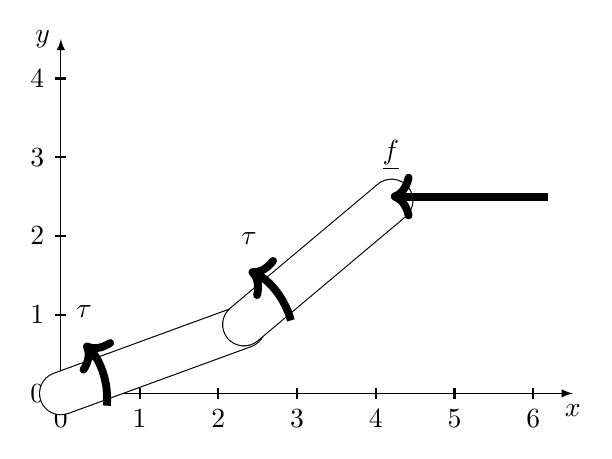
\begin{tikzpicture}
\tkzInit[xmax=6,ymax=4,xmin=0,ymin=0]
%\tkzGrid
\tkzAxeXY
\draw[cm={0.93,0.34,-0.34,0.93,(0,0)}][double=none, double distance=15pt, line join=round, line cap=round] (0.0, 0.0) -- (2.5, 0);
\draw[cm={0.93,0.34,-0.34,0.93,(0, 0)}][->][line width=1mm] (0.5, -0.35) arc (-25:25:1cm) node[ label=above:$\tau$]{ };
\draw[cm={0.75,0.63,-0.63,0.75,(2.325, 0.875)}][double=none, double distance=15pt, line join=round, line cap=round] (0.0, 0.0) -- (2.5, 0);
\draw[cm={0.75,0.63,-0.63,0.75,(2.325, 0.875)}][->][line width=1mm] (0.5, -0.35) arc (-25:25:1cm) node[ label=above:$\tau$]{ };
\draw[->][cm={1.0, 0.0, 0.0, 1.0,(4.19, 2.5)}][line width=1mm] (2.0, 0.0) -- (0.0, 0.0) node[ label=above:$\underline{f}$]{ };;
\end{tikzpicture}
\end{figure}

What $\underline{\tau}$ is required to counteract $\underline{f}$? Since this is a statics analysis, we'll treat the robot as a structure, locking all of the joints. 

Some definitions:
\begin{eqnarray}
\underline{f}_{i} & \text{force exerted on link i by link i-1} \nonumber\\
\underline{n}_{i} & \text{torque exerted in link i by link i-1} \nonumber
\end{eqnarray}

\begin{figure}
	\centering
	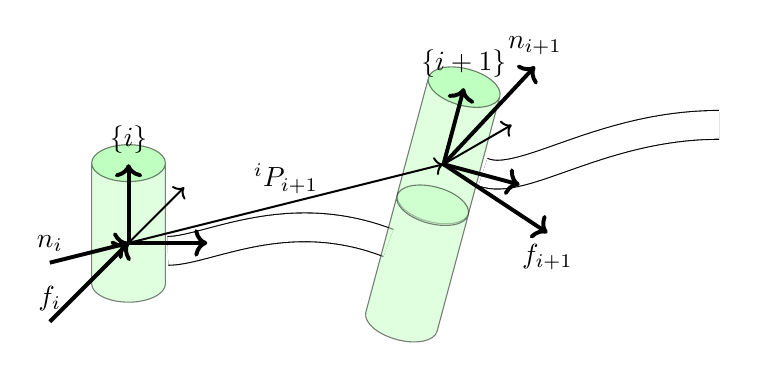
\begin{tikzpicture}
		\coordinate (A) at (0,0);
		\coordinate(B) at (3,1);
		
		\node[cylinder, draw, shape aspect=0.5,cylinder uses custom fill, cylinder end fill=green!50,minimum height=0.5cm,cylinder body fill=green!25, opacity=0.5,scale=4, rotate=90]{};
		\draw[double=none, double distance=10pt, line join=flat, line cap=flat] (0.5, -0.1) .. controls (1.0, -0.1) and (2.0, 0.5) .. (3.3,0);
		\draw[->][line width=0.5mm] (0,0) -- (1,0);
		\draw[->][line width=0.5mm] (0,0) -- (0,1) node[above]{$\{i\}$};
		\draw[->][line width=0.25mm] (0,0) -- (0.707, 0.707);
		\draw[->][line width=0.5mm] (-1, -0.25) node[above]{$n_{i}$} -- (0,0);
		\draw[->][line width=0.5mm] (-1, -1) node[above]{$f_{i}$} -- (0,0);
		\begin{scope}[shift={(4,1)}]
			\coordinate (A) at (0,0);
			\coordinate(B) at (3,1);
	    	\node[cylinder, draw, shape aspect=.5, cylinder uses custom fill, cylinder end fill=green!50, minimum height=0.5cm,cylinder body fill=green!25, opacity=0.5, scale=4, rotate=75]{};
			\draw[double=none, double distance=10pt, line join=flat, line cap=flat] (0.5, -0.1) .. controls (1.0, -0.3) and (2.0, 0.5) .. (3.5,0.5);
			\draw[->][rotate=-15][line width=0.5mm] (0,0) -- (1,0);
			\draw[->][rotate=-15][line width=0.5mm] (0,0) -- (0,1) node[above]{$\{i+1\}$};
			\draw[->][rotate=-15][line width=0.25mm] (0,0) -- (0.707, 0.707);
			\draw[->][rotate=-15][line width=0.5mm] (0,0) -- (0.8,1.5) node[above]{$n_{i+1}$};
			\draw[->][rotate=-15][line width=0.5mm] (0,0) -- (1.5, -0.5) node[below]{$f_{i+1}$};
		\end{scope}	
		\begin{scope}[shift={(3.6,-0.5)}]
			\coordinate (A) at (0,0);
			\coordinate(B) at (3,1);
			\node[cylinder, draw, shape aspect=.5, cylinder uses custom fill, cylinder end fill=green!25, minimum height=0.5cm,cylinder body fill=green!25, opacity=0.5, scale=4, rotate=75]{};
		\end{scope}	
	
		\draw[->][line width=0.25mm] (0,0) -- (4,1) node[pos=0.5,above]{$^{i}P_{i+1}$};
	%	\draw[double=none, double distance=10pt, line join=flat, line cap=flat] (0.8, 0.1) .. controls (1.0, 0) and (2.0, 1.5) .. (3,1);
	
	\end{tikzpicture}
\end{figure}

Since this is a static analysis, we assume that the forces and the torques must add to zero. Specifically,
\begin{displaymath}
^{i}f_{i} - \ \!^{i}f_{i+1} = 0
\end{displaymath}
and
\begin{displaymath}
^{i}n_{i} - \ \!^{i}n_{i+1} - \ \!^{i}P_{i+1} \times \ \!^{i}f_{i+1} = 0
\end{displaymath}
In order to recursively calculate the forces and torques exerted on each link, we have to start with the last link and work backwards, towards the base frame. And we need equations that are formulated entirely in terms of the forces and torques exerted by the distal link. These can easily be seen to be
\begin{eqnarray}
^{i}f_{i} & = & \ \!^{i}f_{i+1} \\
^{i}n_{i} & = & \ \!^{i}n_{i+1} + \ \!^{i}P_{i+1} \times \ \!^{i}f_{i+1}
\end{eqnarray}
We'd really like to express the forces and torques entirely in their ``own'' frames, so we'll rotate them as such:
\begin{eqnarray}
^{i}f_{i} & = & \ \!^{i}_{i+1}R\ \!^{i+1}f_{i+1} \\
^{i}n_{i} & = &  \ \!^{i}_{i+1}R\ \!^{i+1}n_{i+1} + \ \!^{i}P_{i+1} \times \ \!^{i}f_{i+1}
\end{eqnarray}
NOTE that all forces and moment vectors are absorbed by the structure of the arm except for those exerted about the axis of rotation of the joint. So to balance the force/moment equation, we have to isolate the $z$--component. If the joint is revolute, this is $\tau_{i} = \ \!^{i}n_{i}^{T}\ \!^{i}\hat{Z}_{i}$. If the joint is prismatic, this is $\tau_{i} = \ \!^{i}f_{i}^{T}\ \!^{i}\hat{Z}_{i}$.

\subsection{Virtual Work}
The concept here is that work can be expressed in terms of either motion of the joints or motion of the end effector, and that these two terms must be equal. Work is the inner product of a vector force or torque with a vector displacement. In the case of our diagram, this is
\begin{displaymath}
	\underbrace{\mathcal{F} \cdot \delta\mathcal{X}}_{\substack{\text{Cartesian}\\\text{space}}} = \underbrace{\tau \cdot \delta\Theta}_{\substack{\text{Joint}\\ \text{space}}}
\end{displaymath}
where $\mathcal{F}$ is a Cartesian force--moment vector acting on the end effector, $\delta\Theta$ is a infinitesimal Cartesian displacement of the end effector, $\tau$ is the vector of torques at the joints, and $\delta \Theta$ is an infinitesimal vector of joint displacements.

You can write a dot product as a vector multiplication, so
\begin{displaymath}
\underbrace{\mathcal{F}^{T}\delta\mathcal{X}}_{\substack{\text{Cartesian}\\\text{space}}} = \underbrace{\tau^{T} \delta\Theta}_{\substack{\text{Joint}\\ \text{space}}}
\end{displaymath}
Recall that the Jacobian relates infinitesimal motions of the joints to infinitesimal motions of the end effector, e.g. $\delta \mathcal{X} = J \delta\Theta$. So we can write
\begin{displaymath}
\mathcal{F}^{T}J\delta\Theta = \tau^{T}\delta\Theta
\end{displaymath}
And this has to be true for \textbf{any} value of $\delta \Theta$, so we can cancel this term out to get
\begin{displaymath}
\mathcal{F}^{T}J = \tau^{T}
\end{displaymath}
or
\begin{displaymath}
\tau = J^{T}\mathcal{F}
\end{displaymath}

\section{Example}
\begin{figure}[h!]
	\centering
	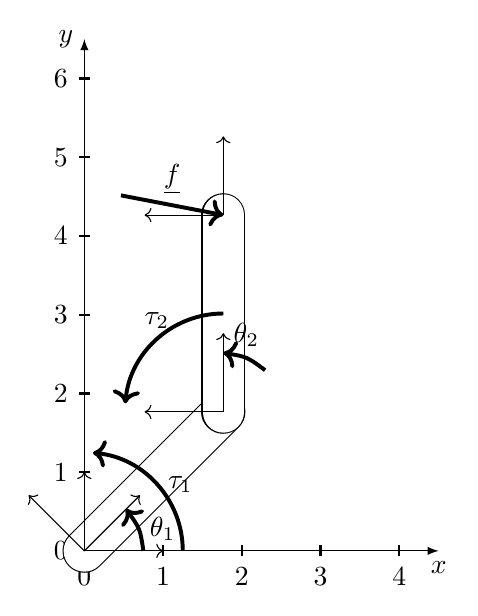
\begin{tikzpicture}
	\tkzInit[xmax=4,ymax=6,xmin=0,ymin=0]
	%\tkzGrid
	\tkzAxeXY
	\draw[cm={0.707,0.707,-0.707,0.707,(0,0)}][double=none, double distance=15pt, line join=round, line cap=round] (0.0, 0.0) -- (2.5, 0);
	\draw[cm={0.707,0.707,-0.707,0.707,(0, 0)}][->] (0.0, 0.0) -- (1.0, 0.0);
	\draw[cm={0.707,0.707,-0.707,0.707,(0, 0)}][->] (0.0, 0.0) -- (0.0, 1.0);
	\draw[cm={0.707,0.707,-0.707,0.707,(0, 0)}][line width=0.5mm][<-] (.75, 0.0) .. controls (0.7, -0.3) .. (0.75*0.707, 0.75*-0.707)  node[pos=0.5,right]{$\theta_{1}$};
	\draw[line width=0.5mm][->] (1.25, 0) arc(0:85:1.25cm) node[pos=0.5,right]{$\tau_{1}$};
	
	\draw[cm={0, 1, -1, 0,(1.765, 1.765)}][double=none, double distance=15pt, line join=round, line cap=round] (0.0, 0.0) -- (2.5, 0);
	\draw[cm={0, 1, -1, 0,(1.765, 1.765)}][->] (0.0, 0.0) -- (1.0, 0.0);
	\draw[cm={0, 1, -1, 0,(1.765, 1.765)}][->] (0.0, 0.0) -- (0.0, 1.0);
	\draw[cm={0, 1, -1, 0,(1.765, 1.765)}][line width=0.5mm][<-] (.75, 0.0) .. controls (0.7, -0.3) .. (0.75*0.707, 0.75*-0.707) node[pos=0.5,above]{$\theta_{2}$};
	\draw[cm={0, 1, -1, 0,(1.765, 1.765)}][line width=0.5mm][->] (1.25, 0) arc(0:85:1.25cm) node[pos=0.5,above]{$\tau_{2}$};

	\draw[->] (0.0, 0.0) -- (1.0, 0.0);
	\draw[->] (0.0, 0.0) -- (0.0, 1.0);
	
	\draw[cm={0, 1, -1, 0, (1.765, 4.265)}][->] (0.0, 0.0) -- (1.0, 0.0);
	\draw[cm={0, 1, -1, 0, (1.765, 4.265)}][->] (0.0, 0.0) -- (0.0, 1.0);
	\draw[cm={1, 0, 0, 1, (1.765, 4.265)}][<-][line width=0.5mm] (0.0, 0.0) -- (-1.3, 0.25) node[pos=0.5,above]{$\underline{f}$};
	\end{tikzpicture}
\end{figure}

Given $\underline{f}$, we want to find $\underline{\tau}$. From our previous result, we know that
\begin{displaymath}
\underline{\tau} = \ \!^{0}J^{T}\ ^{0}\underline{f} = \ \!^{3}J^{T}\ ^{3}\underline{f}
\end{displaymath}
Normally, we get $^{3}\underline{f}$ from a force--torque sensor attached to the end effector, which is in frame 3. We get $^{3}J$ from Equation 5.66. So:
\begin{displaymath}
\underline{\tau} = \left[ \begin{array}{cc} l_{1}s_{2} & 0 \\ l_{1}c_{2} + l_{2} & l_{1}\end{array}\right]^{T}\left[\begin{array}{c} ^{3}f_{x} \\ ^{3}f_{y} \end{array}\right]
\end{displaymath}
or
\begin{eqnarray}
	\tau_{1} & = & l_{1}s_{2}f_{x} + (l_{2}+l_{1}c_{2})f_{y} \nonumber\\
	\tau_{2} & = & l_{2}f_{y} \nonumber
\end{eqnarray}

\section{Cartesian transformation of velocities and forces}
Sometimes we'll want to consider generalized force/moment and translational/rotational velocity vectors, e.g.
\begin{displaymath}
\mathcal{V} = \left[\begin{array}{c}v \\ \omega \end{array}\right]
\end{displaymath}
and
\begin{displaymath}
\mathcal{F} = \left[\begin{array}{c}f \\ n \end{array}\right]
\end{displaymath}
We already have all the machinery we need to write $6 \times 6$ matrix transformations to handle these generalized cases. Specifically, we can rewrite Equations 5.45, 5.47 (for revolute joints):
\begin{eqnarray}
^{i+1}\omega_{i+1} & = & \ \!^{i+1}_{i}R\ \!^{i}\omega_{i} + \dot{\theta}_{i+1}\ \!^{i+1}\hat{Z}_{i+1} \nonumber \\
^{i+1}v_{i+1} & = & \ \!^{i+1}_{i}R\left(\ \!^{i}v_{i} + \ \!^{i}\omega_{i} \times \ \!^{i}P_{i+1}\right) \nonumber
\end{eqnarray}
or equation 5.48 (for prismatic joints):
\begin{eqnarray}
^{i+1}\omega_{i+1} & = & \ \!^{i+1}_{i}R\ \!^{i}\omega_{i} \nonumber \\
^{i+1}v_{i+1} & = & \ \!^{i+1}_{i}R\left(\ \!^{i}v_{i} + \ \!^{i}\omega_{i} \times \ \!^{i}P_{i+1}\right) + \dot{d}_{i+1}\ \!^{i+1}\hat{Z}_{i+1} \nonumber
\end{eqnarray}
IMPORTANT NOTE: we are dealing here with a static situation --- we aren't considering motion of the robot's joints here --- so we can simplify this as
\begin{eqnarray}
^{i+1}\omega_{i+1} & = & \ \!^{i+1}_{i}R\ \!^{i}\omega_{i}  \nonumber \\
^{i+1}v_{i+1} & = & \ \!^{i+1}_{i}R\left(\ \!^{i}v_{i} + \ \!^{i}\omega_{i} \times \ \!^{i}P_{i+1}\right) \nonumber
\end{eqnarray}
and
\begin{eqnarray}
^{i+1}\omega_{i+1} & = & \ \!^{i+1}_{i}R\ \!^{i}\omega_{i} \nonumber \\
^{i+1}v_{i+1} & = & \ \!^{i+1}_{i}R\left(\ \!^{i}v_{i} + \ \!^{i}\omega_{i} \times \ \!^{i}P_{i+1}\right) \nonumber
\end{eqnarray}

By factoring these results and integrating them into a single matrix--vector equation, we get (for revolute joints):
\begin{displaymath}
\left[\begin{array}{c}^{B}v_{B} \\ ^{B}\omega_{B}\end{array}\right] = \left[\begin{array}{cc}^{B}_{A}R & -\ \!^{B}_{A}R\ \!^{A}P_{B,Org}\!\times \\ 0 & ^{B}_{A}R\end{array}\right]\left[\begin{array}{c}^{A}v_{A} \\ ^{A}\omega_{A}\end{array}\right]
\end{displaymath}
for two frames $\{A\}=i$ and $\{B\}=i+1$, where we have expressed the cross product operator in matrix form:
\begin{displaymath}
P\!\times = \left[\begin{array}{ccc} 0 & -p_{z} & p_{y} \\ p_{z} & 0 & -p_{x} \\ -p_{y} & p_{x} & 0 \end{array}\right]
\end{displaymath}
Note also that we have made use of the identity $\omega \times p = -p \times \omega$ in the $(1,2)$ element of this matrix expression.

We will refer to the matrix above as a \textbf{velocity transformation} $T_{v}$:
\begin{displaymath}
^{B}\mathcal{V}_{B} = \ \!^{B}_{A}T_{v}\ \!^{A}\mathcal{V}_{A}.
\end{displaymath}
 Be careful not to confuse this with a generalized coordinate transformation matrix, which is often denoted as $^{i+1}_{i}T\ $!

In exercise 5.1 you are asked to derive the expression for $T_{v}^{-1}$, which is
\begin{displaymath}
\left[\begin{array}{c}^{A}v_{A} \\ ^{A}\omega_{A}\end{array}\right] = \left[\begin{array}{cc}^{A}_{B}R & P_{B,Org}\!\times\ \!^{A}_{B}R\ \!^{A} \\ 0 & ^{A}_{B}R\end{array}\right]\left[\begin{array}{c}^{B}v_{B} \\ ^{B}\omega_{B}\end{array}\right]
\end{displaymath}

And similarly, from Equations 5.80 and 5.81, we can express the generalized force/moment transformation as 
\begin{displaymath}
\left[\begin{array}{c}^{A}f_{A} \\ ^{A}n_{A}\end{array}\right] = \left[\begin{array}{cc}^{A}_{B}R & 0 \\ ^{A}P_{B,Org}\!\times\ \!^{A}_{B}R & ^{A}_{B}R\end{array}\right]\left[\begin{array}{c}^{B}f_{B} \\ ^{B}n_{B}\end{array}\right]
\end{displaymath}
We will refer to the matrix above as a \textbf{force--moment transformation} $T_{f}$:
\begin{displaymath}
^{A}\mathcal{F}_{A} = \ \!^{A}_{B}T_{f}\ \!^{B}\mathcal{F}_{B}.
\end{displaymath}

\subsection{Example}
\begin{figure}[h!]
	\centering
	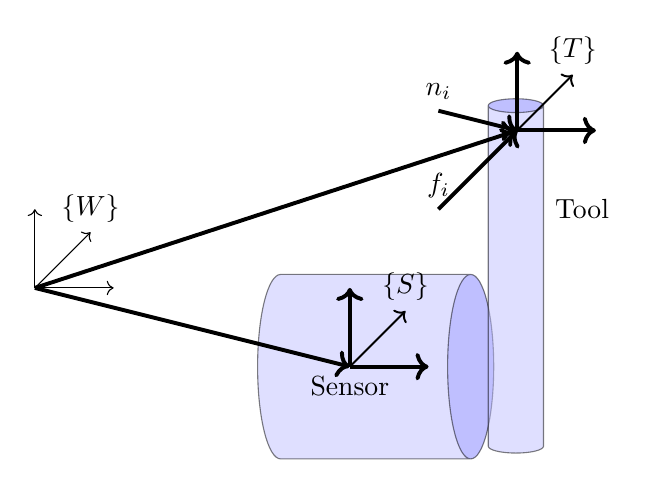
\begin{tikzpicture}
	\coordinate (A) at (0,0);
	\coordinate(B) at (3,1);
	
	\node[cylinder, draw, shape aspect=0.25,cylinder uses custom fill, cylinder end fill=blue!50,minimum height=0.10 cm,cylinder body fill=blue!25, opacity=0.5,scale=10, rotate=0]{}; \node[below]{Sensor};
	\draw[->][line width=0.5mm] (0,0) -- (1,0);
	\draw[->][line width=0.5mm] (0,0) -- (0,1);
	\draw[->][line width=0.25mm] (0,0) -- (0.707, 0.707) node[above]{$\{S\}$};

	\node[cylinder, draw, shape aspect=0.25,cylinder uses custom fill, cylinder end fill=blue!50,minimum height=1.5 cm,cylinder body fill=blue!25, opacity=0.5,scale=3, rotate=90, yshift=-20, xshift=10]{};
	\draw (2.95, 2) node{Tool};
	\draw[->][line width=0.5mm] (2.125,3) -- (3.125,3);
	\draw[->][line width=0.5mm] (2.125,3) -- (2.125,4);
	\draw[->][line width=0.25mm] (2.125,3) -- (0.707+2.125, 0.707+3)  node[above]{$\{T\}$};
	\draw[->][line width=0.5mm] (2.125+-1, 3+0.25) node[above]{$n_{i}$} -- (2.125,3);
	\draw[->][line width=0.5mm] (2.125-1, 3-1) node[above]{$f_{i}$} -- (2.125,3);
	
	\draw[->] (-4, 1) -- (-4, 2);
	\draw[->] (-4, 1) -- (-3, 1);
	\draw[->] (-4, 1) -- (-4+0.707, 1+0.707)  node[above]{$\{W\}$};
	
	\draw[->][line width=0.5mm] (-4,1) -- (2.125,3);
	\draw[->][line width=0.5mm] (-4,1) -- (0,0);
	\end{tikzpicture}
\end{figure}

It's often the case that we will have a force--torque sensor mounted somewhere in the wrist of a robot, but that what we are really interested is the forces and torques applied at the tool tip, not those in the sensor frame. To transform from sensed forces and torques to the tool frame, we calculate $^{T}_{S}T_{f}$:
\begin{displaymath}
	^{T}_{S}T_{f} = \left[ \begin{array}{cc} ^{T}_{S}R & 0 \\ ^{T}P_{S,Org}\times \ \!^{T}_{S}R & ^{T}_{S}R \end{array}\right]
\end{displaymath}
and therefore
\begin{displaymath}
^{T}\mathcal{F}_{T} = \ \!^{T}_{S}T_{f}\ \!^{S}\mathcal{F}_{S}
\end{displaymath}
\end{document}
